\section{Durchführung}
\label{sec:Durchführung}

\subsection{Dewar-Gefäß}
Zunächst muss die Wärmekapazität des Dewar-Gefäß bestimmt werden.
Dafür wird eine bestimmte Wassermenge in das Gefäß gegeben und die Temperatur des Wassers gemessen.
Daraufhin wird eine weitere möglichst gleichgroße Wassermenge erhitzt und ebenfalls in das Gefäß gegeben.
Nun wird das Dewar-Gefäß so gut es geht verschlossen, während die Temperatur des Wassers im Gefäß mit einem Thermometer gemessen wird.
Nach ungefähr 2 Minuten wird die Temperatur des Wassers, welches inzwischen eine homogene Temperatur haben sollte, gemessen und notiert.
Mit der Differenz zwischen Starttemperatur des Wassers und Mischtemperatur des Wassers nach zwei Minuten, kann nun berechnet werden wie viel Wärme das Dewar-Gefäß aufgenommen hat.

\subsection{Messungen der Proben}
Der Versuch wird wie in Abbildung \ref{fig:aufbau} aufgebaut.
Nun wird eine bestimmte Wassermenge in das Dewar-Gefäß gegeben.
Dieses sollte eine möglichst geringe Temperatur haben, damit später ein gut messbarer Temperaturunterschied vorhanden ist.
Die Temperatur des Wasser wird mit einem Thermometer bestimmt und notiert.
Ein weiteres Gefäß wird mit Wasser gefüllt. 
In dieses wird eine Metall Probe gegeben.
Das Gefäß wird, wie in Abbildung \ref{fig:becher} dargestellt, auf eine Heizplatte gestellt, sodass sich das Wasser und die darin enthaltene Probe erhitzt.
Nach einiger Zeit wird die Probe aus dem Behälter genommen, die Temperatur gemessen und in das Dewar-Gefäß gelegt.
Das Gefäß wird nun verschlossen um so wenig Wärme zu verlieren wie möglich.
Im Deckel befindet sich ein kleines Loch durch welches mit einem Thermometer die Temperatur des Wassers im Dewar-Gefäß gemessen wird.
Nach ungefähr zwei Minuten wird die Temperatur notiert und die Probe aus dem Gefäß entnommen.
Daraufhin wird das Wasser im Dewar-Gefäß ausgetauscht und eine neue Probe erhitzt.
Der Messvorgang wird für jede Probe drei mal wiederholt um den Fehler möglichst gering zu halten.
Aus Zeitgründen wurden zwei Proben drei mal gemessen und eine nur ein Mal.
Die genutzten Proben waren Graphit, Blei, und Aluminium. 
\begin{figure}
    \centering
    \caption{Zwei Abbildungen zur Durchführung.}
    \begin{subfigure}{.475\textwidth}
        \centering
        \caption{Der Versuchsaufbau.}
        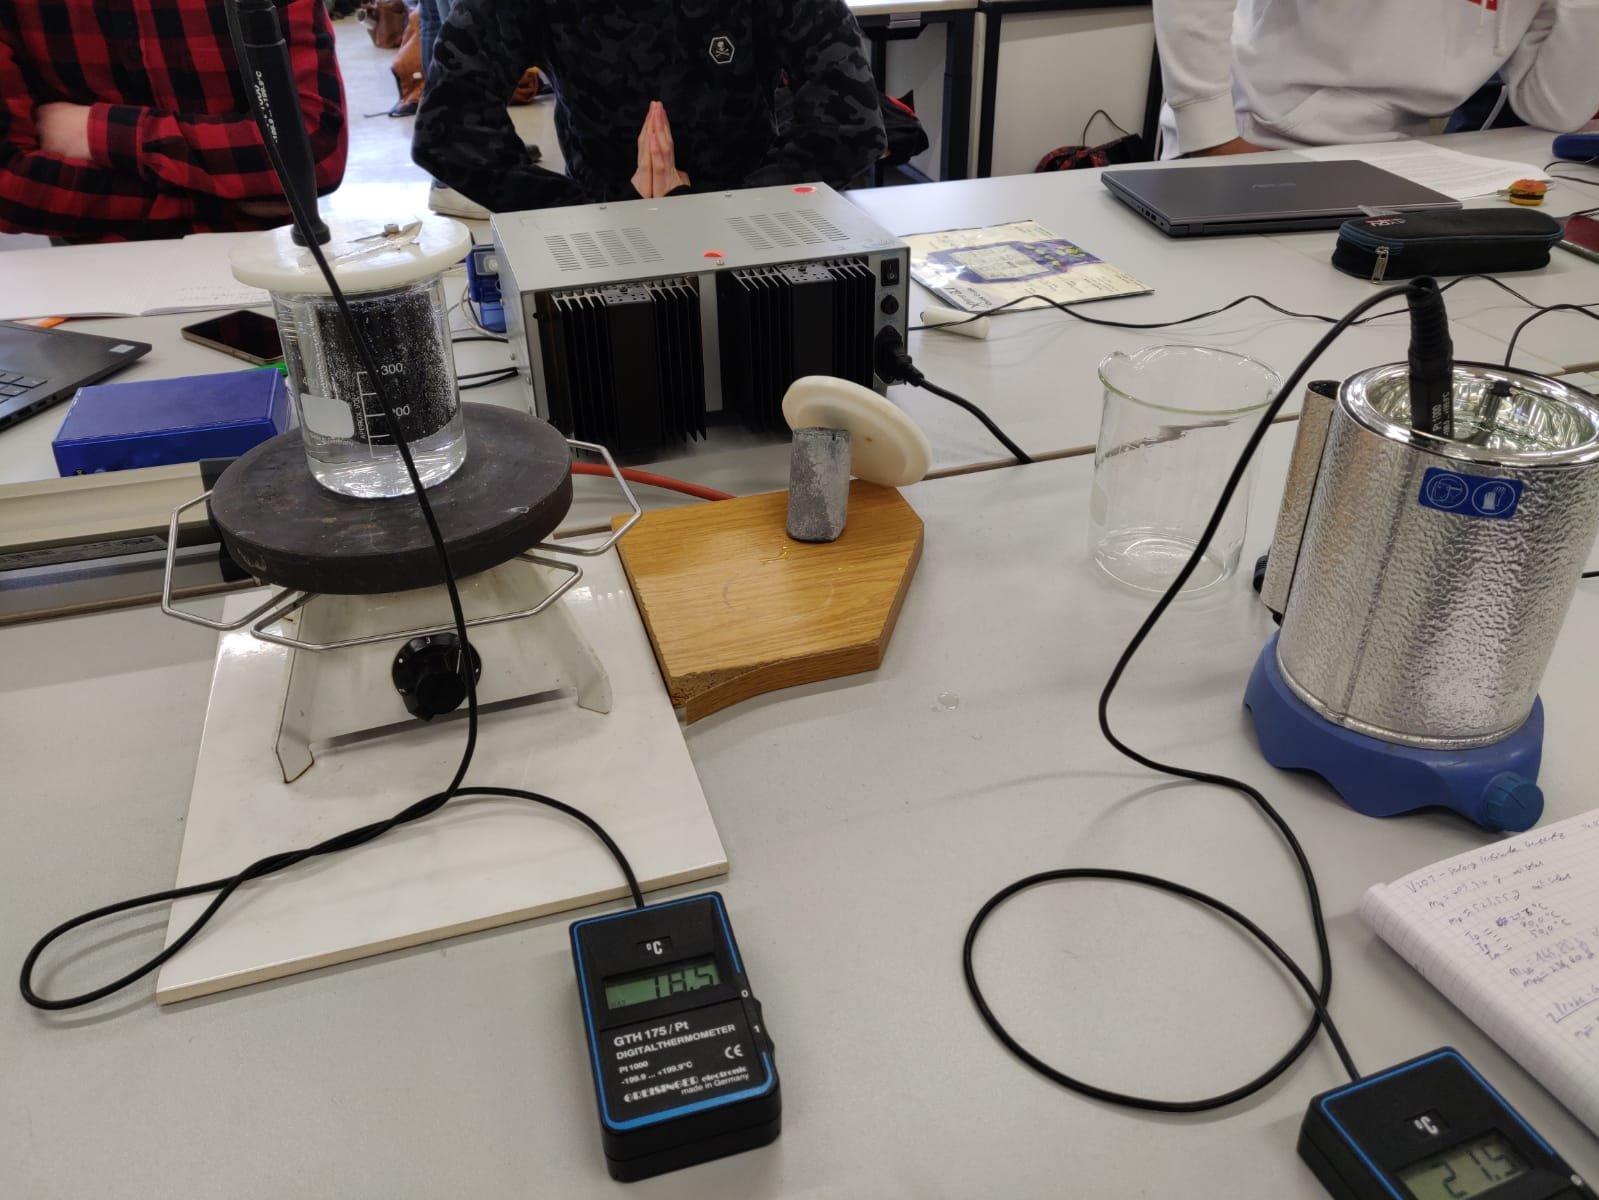
\includegraphics[width=0.7\textwidth]{content/data/Versuchsaufbau.png}
        \label{fig:aufbau}
    \end{subfigure}
    \begin{subfigure}{.475\textwidth}
        \centering
        \caption{Erwärmung der Probe.}
        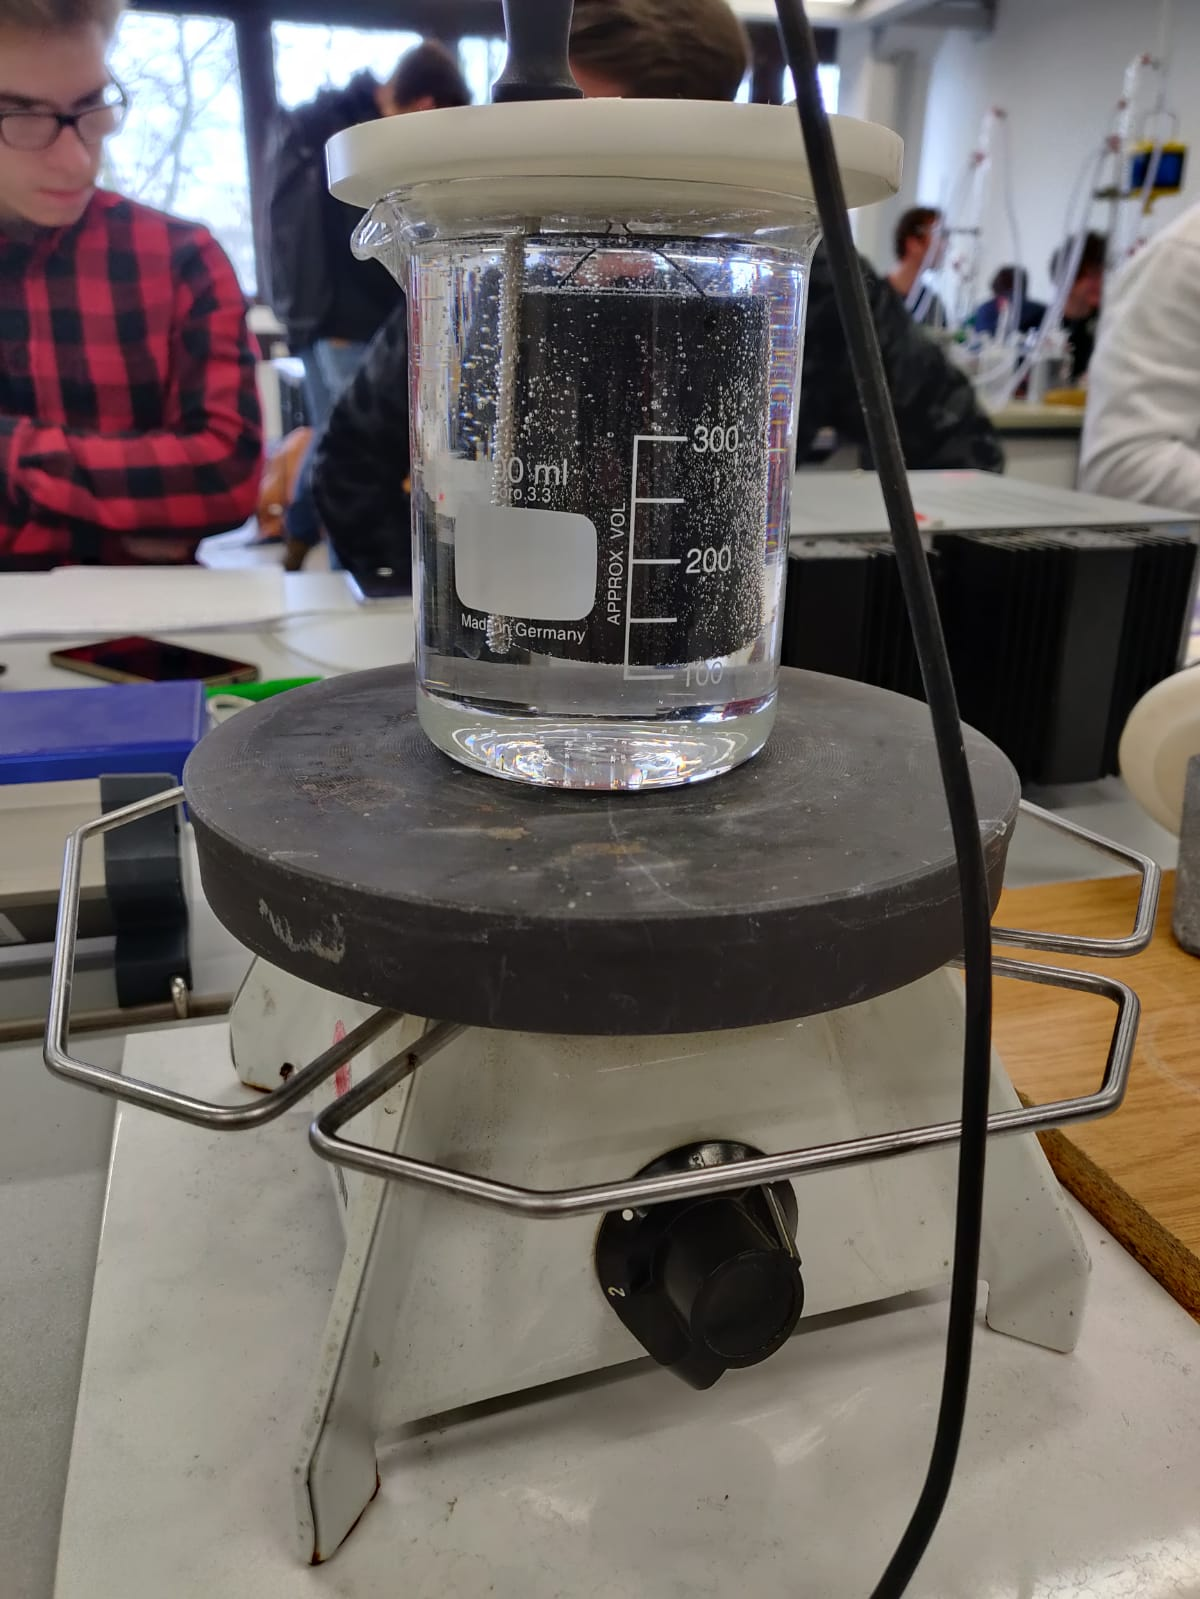
\includegraphics[width=0.7\textwidth]{content/data/Becherglas.png}
        \label{fig:becher}
    \end{subfigure}
    \label{fig:aufbau_allgemein}
\end{figure}